% !TeX root = ../../Book1.tex
% 纲要标题：### 10.1 常曲率模型的度量几何
% 纲要位置：几何学计划纲要.md，第 505 行。
% 正文状态：初稿；尚未正式审核。

% 纲要内容开始
% 
% * 双曲面、圆盘和上半平面
% * 模型间等距映射的构造
% * 距离、测地线及理想边界
% * Möbius 变换与等距群
% * 球面与双曲三角恒等式
% * 角和、面积及曲率归一化
% * 测地多边形和角条件
% 
% 纲要内容结束

\section{常曲率模型的度量几何}
\label{g1:sec:1001}

同样是圆盘，在通常的欧氏度量下，走到边缘只需有限长度；若越靠近边缘，度量把长度放大得越快，边缘就可能变得无限遥远。双曲平面的圆盘模型正是这样的例子。为了看清距离、测地线和对称变换，我们还会把同一几何放在双曲面与上半平面中表达。三个模型各有便于计算的地方，彼此间的显式等距映射使这些计算能够相互转用。

\subsection{双曲面、圆盘和上半平面}
\label{g1:subsec:1001:01}

先取单位球面 \(S^2\subset\mathbb R^3\) 及其诱导度量，它的曲率为 \(1\)。我们寻找一个负曲率的对应模型。把通常内积中的一项改成负号，定义 \(\mathbb R^3\) 上的双线性型
\[
	\langle x,y\rangle_L\coloneqq-x_0y_0+x_1y_1+x_2y_2.
\]
这是\term[lorentzxing]{Lorentz 型}[Lorentzian form]，不是正定内积；例如 \(\langle(1,0,0),(1,0,0)\rangle_L=-1\)。我们并不把它在整个 \(\mathbb R^3\) 上当作长度，而只将它限制到下面曲面的切平面。\footnote{Lorentz，中文常译洛伦兹；Hendrik Antoon Lorentz（1853--1928），荷兰理论物理学家，研究电磁理论、电子理论与运动物体的变换。}

\begin{definition}
	\label{g1:def:hyperbolic-models}
	\term[shuangqumianmoxing]{双曲面模型}[hyperboloid model]是
	\[
		\mathbb H_L^2\coloneqq\{x:\langle x,x\rangle_L=-1,\ x_0>0\},
		\qquad g_L(v,w)=\langle v,w\rangle_L.
	\]
	另外定义\term[yuanpanmoxing]{圆盘模型}[disc model]与\term[shangbanpingmianmoxing]{上半平面模型}[upper half-plane model]：
	\begin{align*}
		\mathbb D&=\{w=u+iv:|w|<1\},&
		g_{\mathbb D}&=\frac{4(\mathrm{d}u^2+\mathrm{d}v^2)}{(1-|w|^2)^2},\\
		\mathbb H&=\{z=x+iy:y>0\},&
		g_{\mathbb H}&=\frac{\mathrm{d}x^2+\mathrm{d}y^2}{y^2}.
	\end{align*}
	复数记号 \(|\mathrm{d}z|^2\) 只简写实二次型 \(\mathrm{d}x^2+\mathrm{d}y^2\)。后两个模型采用平面的标准定向。
\end{definition}

双曲面上的度量确实正定。写 \(x=(x_0,x')\)，则 \(x_0=\sqrt{1+|x'|^2}\)，所以它首先是一个光滑图像。切向量 \(v=(v_0,v')\) 满足 \(x_0v_0=x'\cdot v'\)，从而
\[
	\langle v,v\rangle_L=|v'|^2-\frac{(x'\cdot v')^2}{x_0^2}
	\geq\frac{|v'|^2}{x_0^2}>0\qquad(v\ne0).
\]
这里最后一个严格不等式来自：若 \(v'=0\)，切向条件也使 \(v_0=0\)。因此这个不定型在每个切平面上都给出通常意义的正定长度与角度。它与双曲面作为欧氏空间曲面时的诱导度量不同，不能用欧氏空间中该图像的主曲率代替它的内在曲率。

\ProseParagraphBreak

在上半平面上，\(g_{\mathbb H}=e^{2\phi}(\mathrm{d}x^2+\mathrm{d}y^2)\)，其中 \(\phi=-\log y\)。回忆\eqref{g1:eq:conformal-gauss-curvature}，共形度量的曲率为 \(-e^{-2\phi}(\phi_{xx}+\phi_{yy})\)。这里 \(\phi_{xx}=0\)、\(\phi_{yy}=1/y^2\)，故 \(K=-1\)。圆盘与双曲面是否也给出相同几何，需要下一小节的等距计算，而不能只凭外形或名称判断。

\subsection{模型间等距映射的构造}
\label{g1:subsec:1001:02}

从点 \((-1,0,0)\) 向平面 \(x_0=0\) 投影，会把双曲面上半支送到单位圆盘。这一选择中的 \(-1\) 使投影分母始终为正，也让无穷远处趋向圆周。上半平面到圆盘则用一个把实轴变成圆周的分式映射。

\begin{proposition}[三个模型的等距]
	\label{g1:prop:hyperbolic-model-isometries}
	以下映射均为光滑等距微分同胚：
	\begin{align*}
		P:\mathbb H_L^2&\longrightarrow\mathbb D,&
		P(x)&=\frac{x_1+ix_2}{x_0+1},\\
		C:\mathbb H&\longrightarrow\mathbb D,&
		C(z)&=\frac{z-i}{z+i}.
	\end{align*}
	双曲面的定向取为使 \(P\) 保向的定向；\(C\) 也保持定向。因此三个模型都具有常曲率 \(-1\)，统称为\term[shuangqupingmian]{双曲平面}[hyperbolic plane]。
\end{proposition}
\begin{proof}
	先由 \(x_1^2+x_2^2=x_0^2-1\)，得到 \(|P(x)|^2=(x_0-1)/(x_0+1)<1\)。反解为
	\[
		P^{-1}(u+iv)=\frac{(1+u^2+v^2,\,2u,\,2v)}{1-u^2-v^2}.
	\]
	这给出了互逆的光滑映射。记 \(q=1-u^2-v^2\)、\(a=u\,\mathrm{d}u+v\,\mathrm{d}v\)。对逆映射求导，有
	\[
		\mathrm{d}x_0=\frac{4a}{q^2},\qquad
		\mathrm{d}(x_1,x_2)=\frac{2(\mathrm{d}u,\mathrm{d}v)}q+\frac{4(u,v)a}{q^2}.
	\]
	代入 Lorentz 型，含 \(a^2\) 的系数为 \(16/q^3+16(u^2+v^2-1)/q^4=0\)，剩下 \(4(\mathrm{d}u^2+\mathrm{d}v^2)/q^2\)，正是圆盘度量。

	对 \(C\)，直接算得
	\[
		1-|C(z)|^2=\frac{4y}{|z+i|^2},\qquad
		C'(z)=\frac{2i}{(z+i)^2},\qquad C^{-1}(w)=i\frac{1+w}{1-w}.
	\]
	这些式子证明 \(C\) 恰把上半平面双射到圆盘，且正反映射光滑。复导数乘法把实长度放大 \(|C'(z)|\) 倍，故
	\[
		C^*g_{\mathbb D}
		=\frac{4|C'(z)|^2|\mathrm{d}z|^2}{(1-|C(z)|^2)^2}
		=\frac{|\mathrm{d}z|^2}{y^2}.
	\]
	非零复数乘法的实行列式为其模平方，所以 \(C\) 保向。最后，等距保持内在曲率，这是\cref{g1:thm:theorema-egregium}及其度量表达\eqref{g1:eq:intrinsic-gauss-curvature}的结论，故三个模型的曲率都是 \(-1\)。
\end{proof}

这些坐标图的用途不同：双曲面的线性代数适合距离与三角公式，圆盘适合展示对称性，上半平面的分式变换适合研究群作用。圆盘和上半平面的度量都是欧氏度量乘以一个正函数，因而保留欧氏角度；它们并不保留欧氏长度。

\subsection{距离、测地线及理想边界}
\label{g1:subsec:1001:03}

在连通度量曲面上，用全部连接 \(p,q\) 的分片 \(C^1\) 曲线定义长度距离
\[
	d(p,q)\coloneqq\inf_{\gamma:p\to q}L(\gamma).
\]
三角不等式来自道路拼接，反向参数给出对称性。局部坐标中的正定度量在小闭坐标球上有正的下界，故走出这个球需要正长度，这也保证不同点的距离不为零。前章的径向极小定理只在正常邻域内比较短曲线；对双曲平面，可以利用模型把比较推广到任意两点。

\begin{theorem}[双曲距离与测地线]
	\label{g1:thm:hyperbolic-distance-geodesics}
	双曲面模型中，若 \(p\in\mathbb H_L^2\)、\(v\in \mathrm{T}_p\mathbb H_L^2\) 且 \(\langle v,v\rangle_L=1\)，则所有单位速测地线由
	\begin{equation}
		\label{g1:eq:hyperboloid-geodesic}
		\gamma(t)=p\cosh t+v\sinh t,\qquad t\in\mathbb R
	\end{equation}
	给出。任意两个不同点之间有唯一测地线段，并且它在全部分片 \(C^1\) 连接曲线中最短。三个模型中的距离分别满足
	\begin{align}
		\cosh d(p,q)&=-\langle p,q\rangle_L,
		\label{g1:eq:hyperboloid-distance}\\
		\cosh d(w_1,w_2)&=1+\frac{2|w_1-w_2|^2}{(1-|w_1|^2)(1-|w_2|^2)},
		\label{g1:eq:disc-distance}\\
		\cosh d(z_1,z_2)&=1+\frac{|z_1-z_2|^2}{2\operatorname{Im}z_1\operatorname{Im}z_2}.
		\label{g1:eq:half-plane-distance}
	\end{align}
	双曲平面单连通，其长度距离完备，每个闭有界球紧；每条测地线也都能在整个实数轴上延拓。
\end{theorem}
\begin{proof}
	先说明如何把任意点移到 \(o=(1,0,0)\)。空间坐标 \((x_1,x_2)\) 的旋转保持 Lorentz 型，而矩阵
	\[
		B_r=\begin{pmatrix}\cosh r&\sinh r&0\\\sinh r&\cosh r&0\\0&0&1\end{pmatrix}
	\]
	也保持该型，并把 \(o\) 送到 \((\cosh r,\sinh r,0)\)。任意点都能写成
	\[
		x=(\cosh r,\sinh r\cos\theta,\sinh r\sin\theta),
	\]
	所以这些变换在双曲面上传递；它们保持上半支，因为变换后的第零坐标不可能为零，且上半支连通。其微分保持切平面上的度量，故都是等距。

	双曲面的协变导数可以由 Lorentz 正交投影计算：沿 \(\gamma\) 的切向量场 \(W\) 满足
	\[
		\mathrm{D}_tW=\dot W+\langle\dot W,\gamma\rangle_L\gamma.
	\]
	右边确与 \(\gamma\) 正交；逐项求导内积给出度量相容，交换坐标导数给出无挠性，因此\cref{g1:prop:surface-connection-properties}的唯一性说明它就是度量联络。对单位速曲线，\(\langle\ddot\gamma,\gamma\rangle_L=-1\)，故测地线方程等价于 \(\ddot\gamma=\gamma\)。解这个线性方程即得\eqref{g1:eq:hyperboloid-geodesic}；代入可核验它始终位于上半支且速度为 \(1\)。前章\cref{g1:prop:geodesic-initial-values}的唯一性说明没有遗漏同初值的其他测地线。

	以 \(o\) 为中心，上面的径向参数给出
	\begin{equation}
		\label{g1:eq:hyperbolic-polar-metric}
		g_L=\mathrm{d}r^2+\sinh^2r\,\mathrm{d}\theta^2,\qquad r>0.
	\end{equation}
	这是直接微分 \((\cosh r,\sinh r\cos\theta,\sinh r\sin\theta)\) 所得。任何从 \(o\) 到径向坐标 \(r_0\) 的曲线，其速度不小于径向速度的绝对值。为避开 \(r=0\) 的极坐标奇点，取 \(0<\varepsilon<r_0\)，只比较曲线最后一次离开 \(r=\varepsilon\) 后的一段，得到长度至少为 \(r_0-\varepsilon\)；让 \(\varepsilon\) 趋零，便得下界 \(r_0\)。固定 \(\theta\) 的径向测地段达到该下界。

	将任意起点 \(p\) 等距移到 \(o\)，可知两点间距离是 \(\operatorname{arcosh}(-\langle p,q\rangle_L)\)。当 \(p\ne q\) 时记它为 \(a>0\)，则到达 \(q\) 的单位初速度必须是
	\[
		v=\frac{q-p\cosh a}{\sinh a}.
	\]
	该向量与 \(p\) 正交且 Lorentz 长度为 \(1\)，于是相应测地段存在且唯一。双曲面测地线的轨迹是过原点的二维平面与上半支之交，且每条单位速参数线都不重复。将 \(P^{-1}\) 代入 Lorentz 内积，整理即得\eqref{g1:eq:disc-distance}；再用
	\[
		|C(z_1)-C(z_2)|^2=\frac{4|z_1-z_2|^2}{|z_1+i|^2|z_2+i|^2}
	\]
	及上一小节的 \(1-|C(z)|^2\) 公式，得到\eqref{g1:eq:half-plane-distance}。

	由距离公式，\(o\) 的半径 \(R\) 闭球恰是双曲面上 \(x_0\leq\cosh R\) 的部分，它在 \(\mathbb R^3\) 中闭且有界，故紧。距离公式又说明坐标收敛蕴含距离收敛；反过来，将极限点移到 \(o\)，由 \(x_0=\cosh r\)、\(|x'|=\sinh r\) 可知距离收敛蕴含坐标收敛。因此上述紧性也是长度距离的紧性。任意 Cauchy 序列有界，落在某个这样的紧球内，有收敛子列，再由 Cauchy 条件整个序列收敛，故度量完备。公式\eqref{g1:eq:hyperboloid-geodesic}另已直接给出测地线的全时延拓；这里没有把两种完备性未经证明地互换。最后，圆盘凸且可沿直线缩到原点，故单连通，模型间的微分同胚将这一性质传给双曲面和上半平面。
\end{proof}

圆盘中的测地线是直径或与单位圆周正交的圆弧。具体地，双曲面测地线所在平面可写为 \(a_0x_0+a_1x_1+a_2x_2=0\)，投影后成为
\[
	a_0(1+u^2+v^2)+2a_1u+2a_2v=0.
\]
当 \(a_0=0\) 时是过原点的直线；否则圆心为 \((-a_1/a_0,-a_2/a_0)\)，半径平方等于圆心到原点距离平方减去 \(1\)，这正是与单位圆正交的条件。每条相交圆弧都对应一个这样的测地平面。把 \(w=C(z)\) 代入，方程化成 \(A(x^2+y^2)+Bx+C_0=0\)，所以在上半平面中，它们是以实轴上点为圆心的半圆，或垂直实轴的直线。通过两个不同内点的这类弧唯一，正与定理的唯一性一致。

\begin{figure}[htbp]
	\centering
	% !TeX root = ../Book1.tex
\begin{tikzpicture}[>=stealth,font=\small]
	\begin{scope}[yshift=1.5cm]
		\draw[dashed,gray] (0,0) circle (1.5);
		\draw[blue!70!black,thick] (-1.5,0)--(1.5,0);
		\draw[blue!70!black,thick] ({1.5*cos(55)},{1.5*sin(55)}) arc[start angle=145,end angle=215,radius={1.5*tan(55)}];
		\fill[gray] ({1.5*cos(55)},{1.5*sin(55)}) circle (1.3pt);
		\fill[gray] ({1.5*cos(55)},{-1.5*sin(55)}) circle (1.3pt);
		\node[above left] at (-.9,1.25) {\(\partial_\infty\mathbb H^2\)};
		\node at (0,-1.95) {圆盘模型};
	\end{scope}
	\draw[->] (3.05,1.55)--(2.05,1.55) node[midway,above] {\(C\)};
	\begin{scope}[xshift=5cm]
		\draw[dashed,gray,->] (-1.65,0)--(1.7,0) node[right] {\(\mathbb R\)};
		\draw[blue!70!black,thick] (-1.35,0) arc[start angle=180,end angle=0,radius=1.05];
		\draw[blue!70!black,thick,->] (1.05,0)--(1.05,2.75) node[above] {\(\infty\)};
		\fill[gray] (-1.35,0) circle (1.3pt);
		\fill[gray] (.75,0) circle (1.3pt);
		\fill[gray] (1.05,0) circle (1.3pt);
		\node at (0,-.45) {上半平面模型};
	\end{scope}
\end{tikzpicture}

	\caption[双曲平面的测地线与理想边界]{圆盘中的测地线为直径及正交于圆周的圆弧；上半平面中则为垂直实轴的直线及圆心在实轴上的半圆。灰色边界用于表示理想端点，不属于模型本身。图中的两组曲线分别示意各模型中的形状，不标示逐条对应。}
	\label{g1:fig:hyperbolic-model-geodesics}
\end{figure}

圆盘的圆周称为其\term[lixiangbianjie]{理想边界}[ideal boundary]，记为 \(\partial_\infty\mathbb H^2\)。上半平面的相应边界是 \(\mathbb R\cup\{\infty\}\)，其中一点 \(\infty\) 由 \(C\) 送到圆周上的 \(1\)。理想端点只描述测地线向哪个方向无限延伸，不是度量完备化中缺少的点。事实上
\[
	d_{\mathbb D}(0,w)=2\operatorname{artanh}|w|
	=\log\frac{1+|w|}{1-|w|}\longrightarrow\infty\qquad(|w|\to1).
\]
双曲面上，同一个端点由向量 \(p+v\) 的正比例类表示，因为\eqref{g1:eq:hyperboloid-geodesic}在 \(t\to+\infty\) 时沿 \(e^t(p+v)/2\) 增长，而 \(\langle p+v,p+v\rangle_L=0\)。不同理想端点恰好确定一条完整测地线；在上半平面中，两有限端点决定一个半圆，有一个端点为 \(\infty\) 时则决定一条竖线。

\ProseParagraphBreak

球面的距离提供了重要对照。\cref{g1:exm:sphere-geodesics}已证明单位球面的测地线是大圆，而且可全时延拓。固定 \(p\in S^2\)，写 \(q=p\cos r+u\sin r\)，其中 \(u\perp p\)、\(|u|=1\)、\(0<r<\pi\)。直接微分给出 \(\mathrm{d}r^2+\sin^2r\,\mathrm{d}\theta^2\)，同样的径向长度比较得到
\begin{equation}
	\label{g1:eq:spherical-distance}
	d_{S^2}(p,q)=\arccos(p\cdot q)\in[0,\pi].
\end{equation}
到对径点时可先截到 \(r=\pi-\varepsilon\) 再取极限，故同一公式仍成立。非对径的不同点之间，较短大圆弧是唯一最短测地段；对径点之间所有半大圆都最短。距离公式还说明它与球面原有拓扑相同，因此球面的紧性保证度量完备以及闭球紧。球面单连通已由\cref{g1:prop:sphere-simply-connected}证明；欧氏平面的相应三种性质则分别来自凸性、欧氏 Cauchy 序列收敛和闭有界集紧性。

\subsection{Möbius 变换与等距群}
\label{g1:subsec:1001:04}

已经知道模型之间怎样等距，现在要找同一模型的全部等距。仅写出一族保持度量的公式还不够，还须证明没有遗漏。一个实用的办法是先证明：等距只要在一点具有相同的位置和微分，便处处相同；随后用显式变换实现所有可能的初始数据。

\begin{proposition}[等距的初始数据]
	\label{g1:prop:isometry-initial-data}
	设 \(M,N\) 是光滑度量曲面，\(M\) 连通，\(F_1,F_2:M\to N\) 为局部等距。若在某一点 \(p\) 有 \(F_1(p)=F_2(p)\) 且 \(\mathrm{d}(F_1)_p=\mathrm{d}(F_2)_p\)，则 \(F_1=F_2\)。特别地，两个局部等距若在非空开集上相同，就在其连通公共定义域上相同。
\end{proposition}
\begin{proof}
	局部等距保持联络：在可逆邻域上，把目标联络拉回源曲面，所得运算满足度量相容、无挠性及求导法则，故由\cref{g1:prop:surface-connection-properties}的唯一性，等于源联络。因此它把带原仿射参数的测地线映为测地线。\cref{g1:prop:geodesic-initial-values}的初值唯一性给出
	\[
		F_i(\exp_qv)=\exp_{F_i(q)}\bigl(\mathrm{d}(F_i)_qv\bigr)
	\]
	对充分小的 \(v\) 成立。

	令 \(S\) 为两映射的位置与微分都相同的点集。假设使它非空。若 \(q\in S\)，由\cref{g1:prop:normal-neighborhood}，\(\exp_q\) 在零附近给出一个开邻域坐标，上式使两映射在整个邻域相同，其微分自然也相同，故 \(S\) 开。若 \(q_j\in S\) 且 \(q_j\to q\)，连续性先给出 \(F_1(q)=F_2(q)\)；在该公共像点附近选一张坐标图，再用两映射的一阶导数连续性，得到 \(\mathrm{d}(F_1)_q=\mathrm{d}(F_2)_q\)，故 \(S\) 闭。连通性迫使 \(S=M\)。
\end{proof}

以下的等距指保持度量的光滑微分同胚，组成等距群 \(\operatorname{Isom}\)。取实矩阵 \(A=\begin{psmallmatrix}a&b\\c&d\end{psmallmatrix}\) 且 \(ad-bc=1\)，定义\term[mobiusbianhuan]{Möbius 变换}[Möbius transformation]
\[
	f_A(z)=\frac{az+b}{cz+d}.
\]
分母在上半平面不为零。其在实轴及 \(\infty\) 上的取值按分式极限解释，例如 \(c\ne0\) 时 \(f_A(\infty)=a/c\)。

\begin{theorem}[双曲平面的等距群]
	\label{g1:thm:hyperbolic-isometry-group}
	上半平面的全部保向等距恰为上述实 Möbius 变换，且
	\[
		\operatorname{Isom}^+(\mathbb H)
		\cong\operatorname{PSL}(2,\mathbb R)
		=\operatorname{SL}(2,\mathbb R)/\{I,-I\}.
	\]
	它在正向正交单位标架上传递，且实现任意给定的源标架与目标标架的等距唯一。全部反向等距都是保向等距与 \(\sigma(z)=-\overline z\) 的复合。圆盘模型的全部保向等距可写成
	\[
		w\longmapsto e^{i\theta}\frac{w-a}{1-\overline a w},\qquad |a|<1,\quad\theta\in\mathbb R.
	\]
\end{theorem}
\begin{proof}
	直接计算有
	\[
		\operatorname{Im}f_A(z)=\frac{y}{|cz+d|^2},\qquad
		f_A'(z)=\frac1{(cz+d)^2}.
	\]
	于是 \(|\mathrm{d}f_A|^2/(\operatorname{Im}f_A)^2=|\mathrm{d}z|^2/y^2\)。逆矩阵给出逆映射，非零复导数保持定向，故它们都是保向等距。代入分式可得 \(f_A\circ f_B=f_{AB}\)。若 \(f_A(z)=z\) 恒成立，比较多项式 \(az+b=cz^2+dz\) 的系数，得到 \(b=c=0\)、\(a=d\)，再由行列式为 \(1\) 得 \(A=\pm I\)，这解释了商群中的两个矩阵。

	对点 \(x+iy\)，映射 \(z\mapsto x+yz\) 将 \(i\) 送到它，对应矩阵
	\[
		\begin{pmatrix}\sqrt y&x/\sqrt y\\0&1/\sqrt y\end{pmatrix}.
	\]
	而矩阵 \(K_t=\begin{psmallmatrix}\cos t&\sin t\\-\sin t&\cos t\end{psmallmatrix}\) 对应的变换固定 \(i\)，其在 \(i\) 处的微分为复数乘法 \(e^{2it}\)，可以实现任意角度的旋转。组合这两类变换及其逆，就能将任意一点的正向单位标架送到任意另一标架。

	现在给定任意保向等距 \(F\)，在一个点选正向单位标架，并从上述变换中选 \(f_A\) 与 \(F\) 的像点和微分一致。\cref{g1:prop:isometry-initial-data}迫使二者处处相同，也证明给定标架数据后的唯一性。反射 \(\sigma\) 保持 \(y\) 与欧氏长度，故是反向等距；任意反向等距与它复合后保向，因而没有其他类型。

	圆盘中的 \(h_a(w)=(w-a)/(1-\overline a w)\) 满足
	\[
		1-|h_a(w)|^2=\frac{(1-|a|^2)(1-|w|^2)}{|1-\overline a w|^2},\qquad
		h_a'(w)=\frac{1-|a|^2}{(1-\overline a w)^2}.
	\]
	所以它是把 \(a\) 送到 \(0\) 的保向等距；其逆为 \(h_{-a}\)。旋转 \(w\mapsto e^{i\theta}w\) 也保持度量，并在 \(0\) 处实现所有正向正交微分。给定保向等距 \(F\)，取 \(a=F^{-1}(0)\)，则 \(F\circ h_a^{-1}\) 固定原点，用初始数据命题知它必为某个旋转，得到所列公式。
\end{proof}

等长的有序双曲线段可以由唯一保向等距相互匹配。确切地，若 \(p\ne q\)、\(p'\ne q'\) 且 \(d(p,q)=d(p',q')\)，取各自唯一最短段的初始单位切向量 \(v,v'\)，将 \((p,v,Jv)\) 送到 \((p',v',Jv')\) 的等距便把整个线段及终点一起送过去；反过来，匹配有序端点的保向等距必须具有这些初始数据。这个结论以后将用于基本多边形的边配对。

\ProseParagraphBreak

球面与欧氏平面也有同样的标架描述。把三个模型的结论统一写出，可以直接用于下一节的边配对及局部几何图册。

\begin{proposition}[模型等距的初始数据]
	\label{g1:prop:model-isometry-data}
	令 \(X\) 为欧氏平面、单位球面或曲率 \(-1\) 的双曲平面。给定 \(p,q\in X\) 及线性内积等距 \(L:\mathrm{T}_pX\to \mathrm{T}_qX\)，存在唯一全局等距 \(F:X\to X\)，使 \(F(p)=q\)、\(\mathrm{d}F_p=L\)。这里允许 \(L\) 保向或反向。因而三个模型的等距群都在同向单位标架上传递，并可用反向等距匹配相反定向的标架。定义在非空连通开集 \(U\subset X\) 上的任意局部等距 \(f:U\to X\)，都有唯一的全局模型等距延拓。
\end{proposition}
\begin{proof}
	双曲情形，保向初值由\cref{g1:thm:hyperbolic-isometry-group}的标架传递性实现；反向初值先与模型反射的微分复合，化成保向初值，再把反射复合回来即可。球面情形，选取 \(\mathrm{T}_pS^2\) 的正交基 \((e_1,e_2)\)。\((p,e_1,e_2)\) 与 \((q,Le_1,Le_2)\) 都是 \(\mathbb R^3\) 的正交基，唯一将前者送到后者的正交线性变换限制到球面，就实现了所需初值；当 \(L\) 保向时矩阵行列式为 \(1\)，反向时为 \(-1\)。欧氏平面则直接取 \(F(x)=q+L(x-p)\)。

	唯一性由\cref{g1:prop:isometry-initial-data}给出。对于局部等距 \(f\)，取 \(p\in U\)，以 \(q=f(p)\)、\(L=\mathrm{d}f_p\) 构造全局等距 \(F\)；同一唯一性命题应用于连通域 \(U\)，便得 \(F|_U=f\)，任何另一全局延拓也具有相同初始数据。
\end{proof}

这还给出了另外两个模型的全部等距：球面保向等距群是 \(\operatorname{SO}(3)\)，全等距群是 \(\operatorname{O}(3)\)；欧氏平面的全等距为 \(x\mapsto Qx+b\)，其中 \(Q\in\operatorname{O}(2)\)，保向时 \(\det Q=1\)。

\subsection{球面与双曲三角恒等式}
\label{g1:subsec:1001:05}

三角公式比较的是边长与角，不依赖画出的曲线看起来有多弯。在双曲平面中，取三个不共测地线的点，以唯一测地段连接；球面中则取包含在一个开半球内的凸测地三角形，三边都用较短大圆弧。记顶点为 \(A,B,C\)，对应内角为 \(\alpha,\beta,\gamma\)，其对边长分别为 \(a,b,c\)。这些条件使三角形非退化，所有角属于 \((0,\pi)\)；球面的边长还属于 \((0,\pi)\)。

\ProseParagraphBreak

双曲三角形确实围成凸圆盘，可以用一个辅助投影看清。令 \(Q(x)=(x_1/x_0,x_2/x_0)\)，则 \(Q\) 把双曲面微分同胚地送到单位圆盘，逆映射为 \(u\mapsto(1,u)/\sqrt{1-|u|^2}\)。测地线所在的过原点平面在该投影下成为直线，故三条测地边恰对应普通三角形的三条线段。这称为\term[kleinmoxing]{Klein 模型}[Klein model]；它使凸性清楚，却一般不保欧氏角度。球面开半球向其切向平面的中心投影同样把较短大圆段变为直线段，所以本节所取的球面三角形也有清楚的凸内部。

\begin{theorem}[常曲率三角公式]
	\label{g1:thm:constant-curvature-trigonometry}
	对上述非退化双曲三角形，曲率为 \(-1\) 时有
	\begin{align}
		\cosh a&=\cosh b\cosh c-\sinh b\sinh c\cos\alpha,
		\label{g1:eq:hyperbolic-cosine-law}\\
		\frac{\sin\alpha}{\sinh a}&=\frac{\sin\beta}{\sinh b}=\frac{\sin\gamma}{\sinh c},
		\label{g1:eq:hyperbolic-sine-law}\\
		\cos\alpha&=-\cos\beta\cos\gamma+\sin\beta\sin\gamma\cosh a.
		\label{g1:eq:hyperbolic-angle-cosine-law}
	\end{align}
	对上述单位球面上的凸三角形，有
	\begin{align}
		\cos a&=\cos b\cos c+\sin b\sin c\cos\alpha,
		\label{g1:eq:spherical-cosine-law}\\
		\frac{\sin\alpha}{\sin a}&=\frac{\sin\beta}{\sin b}=\frac{\sin\gamma}{\sin c},
		\label{g1:eq:spherical-sine-law}\\
		\cos\alpha&=-\cos\beta\cos\gamma+\sin\beta\sin\gamma\cos a.
		\label{g1:eq:spherical-angle-cosine-law}
	\end{align}
	各余弦公式也可按 \((a,\alpha),(b,\beta),(c,\gamma)\) 循环置换。
\end{theorem}
\begin{proof}
	先看双曲面。令 \(u,v\in \mathrm{T}_A\mathbb H_L^2\) 分别为从 \(A\) 指向 \(B,C\) 的单位切向量，故 \(\langle u,v\rangle_L=\cos\alpha\)。测地线公式给出
	\[
		B=A\cosh c+u\sinh c,\qquad
		C=A\cosh b+v\sinh b.
	\]
	取负 Lorentz 内积，利用 \(\langle A,A\rangle_L=-1\)、\(u,v\perp_L A\)，立刻得到\eqref{g1:eq:hyperbolic-cosine-law}。球面情形改用 \(B=A\cos c+u\sin c\)、\(C=A\cos b+v\sin b\)，并取通常内积，就得到\eqref{g1:eq:spherical-cosine-law}。这两个计算解释了公式中双曲余弦与普通余弦、以及中间正负号的区别。

	为证明正弦公式，取 \(\mathcal D=|\det(A,B,C)|\)。在双曲情形，扩充 \(A\) 为 Lorentz 正交单位基 \((A,e_1,e_2)\)，其行列式绝对值为 \(1\)：对基矩阵的关系 \(F^{\mathsf T}\operatorname{diag}(-1,1,1)F=\operatorname{diag}(-1,1,1)\) 取行列式即可看出。上述表达式遂给出
	\[
		\mathcal D=\sinh b\sinh c\sin\alpha
		=\sinh c\sinh a\sin\beta
		=\sinh a\sinh b\sin\gamma.
	\]
	三个角都在 \((0,\pi)\)，故正弦为正，没有额外绝对值符号。除以 \(\sinh a\sinh b\sinh c\) 得所求结论。球面用通常正交基作同样的行列式计算，把各 \(\sinh\) 换成 \(\sin\)，也得到正弦公式。

	最后证明角形式的余弦公式，以免在后面使用直角三角形时暗加另一条恒等式。双曲情形记 \(x=\cosh a\)、\(y=\cosh b\)、\(z=\cosh c\)。将三个位置向量的 Lorentz Gram 矩阵取行列式，得到
	\[
		\mathcal D^2=1+2xyz-x^2-y^2-z^2.
	\]
	边余弦公式给出 \(\cos\beta=(xz-y)/(\sinh a\sinh c)\)、\(\cos\gamma=(xy-z)/(\sinh a\sinh b)\)，行列式公式给出对应的正弦。于是 \(-\cos\beta\cos\gamma+x\sin\beta\sin\gamma\) 的共同分子为
	\[
		-(xz-y)(xy-z)+x\mathcal D^2=(x^2-1)(yz-x),
	\]
	共同分母为 \((x^2-1)\sinh b\sinh c\)。约去后是 \(\cos\alpha\)，证明\eqref{g1:eq:hyperbolic-angle-cosine-law}。

	球面情形令 \(x=\cos a\)、\(y=\cos b\)、\(z=\cos c\)，通常 Gram 行列式仍给出同一个 \(\mathcal D^2\) 表达式；这时相应分子为
	\[
		-(y-xz)(z-xy)+x\mathcal D^2=(1-x^2)(x-yz),
	\]
	分母为 \((1-x^2)\sin b\sin c\)，约去后仍为 \(\cos\alpha\)。
\end{proof}

例如双曲直角三角形的直角对边为 \(c\) 时，\(\cosh c=\cosh a\cosh b\)；球面对应式为 \(\cos c=\cos a\cos b\)。这些是相应的勾股关系。若边长都很小，把 \(\cosh t=1+t^2/2+O(t^4)\)、\(\sinh t=t+O(t^3)\) 代入双曲余弦公式，最低阶便恢复 \(a^2=b^2+c^2-2bc\cos\alpha\)。局部接近欧氏几何，并不意味着这些公式对较大三角形仍可用欧氏公式替代。

\subsection{角和、面积及曲率归一化}
\label{g1:subsec:1001:06}

三角公式通过线性代数计算边和角，面积则由前章的曲率积分直接给出。这里必须使用测地边，因为一般曲线边还带有测地曲率积分。

\begin{proposition}[测地多边形的面积]
	\label{g1:prop:geodesic-polygon-area}
	设常曲率 \(K\) 的光滑度量曲面中，紧闭圆盘区域 \(D\) 的边界由 \(n\) 条测地线弧组成，边只在相邻端点相交，各内角 \(\alpha_j\in(0,2\pi)\)。则
	\begin{equation}
		\label{g1:eq:constant-curvature-polygon-area}
		K\operatorname{Area}(D)=\sum_{j=1}^n\alpha_j-(n-2)\pi.
	\end{equation}
	尤其在曲率 \(-1\) 的双曲平面中，面积为 \((n-2)\pi-\sum_j\alpha_j\)；单位球面上面积为 \(\sum_j\alpha_j-(n-2)\pi\)。
\end{proposition}
\begin{proof}
	\cref{g1:thm:global-gauss-bonnet}允许圆盘不在单张坐标图内。这里圆盘的 Euler 示性数为 \(1\)，每条测地边的 \(k_g=0\)，外角是 \(\pi-\alpha_j\)，故
	\[
		K\operatorname{Area}(D)+\sum_{j=1}^n(\pi-\alpha_j)=2\pi.
	\]
	整理即得公式。全部假设中的紧性、圆盘拓扑以及非退化角点，正是所引公式在这里所需的条件。
\end{proof}

非退化双曲三角形有正面积，所以角和严格小于 \(\pi\)；单位球面的上述凸三角形角和严格大于 \(\pi\)。这与\cref{g1:cor:geodesic-triangle-defect}相符。反过来，仅知道三角形某些角度满足一个数值不等式，还不能在未经构造时断言所需边长与边界都已经存在。

\begin{example}[理想三角形]
	\label{g1:exm:ideal-triangle-area}
	在上半平面取理想顶点 \(0,1,\infty\)。它的三边是 \(x=0\)、\(x=1\) 与直径为 \([0,1]\) 的半圆，内部为 \(0<x<1\)、\(y>\sqrt{x(1-x)}\)。面积元是 \(y^{-2}\,\mathrm{d}x\,\mathrm{d}y\)，故
	\[
		\operatorname{Area}(D)
		=\int_0^1\int_{\sqrt{x(1-x)}}^\infty\frac{\mathrm{d}y\,\mathrm{d}x}{y^2}
		=\int_0^1\frac{\mathrm{d}x}{\sqrt{x(1-x)}}=\pi.
	\]
	最后可令 \(x=(1+\cos t)/2\) 积分。这个区域非紧，其顶点也不在双曲平面内，因此不能不加解释地把角度 \(0\) 代入紧圆盘定理；这里的直接积分给出了依据。任意三个不同且按正向排列的理想端点都可由实分式变换送到 \(0,1,\infty\)：若三者有限，先用 \((z-a)(b-c)/((z-c)(b-a))\) 把它们送到 \(0,1,\infty\)，涉及 \(\infty\) 时取相应极限，选择保持边界循环次序的排列保证它保持上半平面；矩阵再归一化为行列式 \(1\)。所以每个理想三角形的面积都是 \(\pi\)。
\end{example}

曲率的归一化会改变面积公式中的尺度。若把度量乘以常数 \(R^2>0\)，长度乘以 \(R\)，面积乘以 \(R^2\)，角度不变。\eqref{g1:eq:christoffel-metric}中度量与逆度量的常数因子相消，所以联络不变；\eqref{g1:eq:intrinsic-gauss-curvature}的分子乘以 \(R^2\)、分母乘以 \(R^4\)，故曲率乘以 \(R^{-2}\)。因此半径 \(R\) 的球面与曲率 \(-1/R^2\) 的双曲平面，三角公式中的每个边长都应写成 \(a/R,b/R,c/R\)，而面积公式分别成为
\[
	\operatorname{Area}_{+}(D)=R^2\left(\sum_j\alpha_j-(n-2)\pi\right),\qquad
	\operatorname{Area}_{-}(D)=R^2\left((n-2)\pi-\sum_j\alpha_j\right).
\]
两式中的角度都以弧度计。选定曲率 \(-1\) 相当于选定长度单位，并非说任意常负曲率度量的数字都天然等于 \(-1\)。

\subsection{测地多边形和角条件}
\label{g1:subsec:1001:07}

为了随后把多边形的边两两粘合，需要能同时控制边长与顶点内角。欧氏正 \(n\) 边形缩放后角度不变；双曲正 \(n\) 边形则会随大小增加而使内角减小。这一变化恰好提供了曲面粘合所需的角度。

\begin{proposition}[正则双曲多边形]
	\label{g1:prop:regular-hyperbolic-polygons}
	对整数 \(n\geq3\) 及任意
	\[
		0<\alpha<\frac{(n-2)\pi}{n},
	\]
	曲率 \(-1\) 的双曲平面中存在一个凸正则测地 \(n\) 边形，其边长相等、内角均为 \(\alpha\)。以中心到顶点的距离 \(R>0\) 作参数时，内角恰为
	\begin{equation}
		\label{g1:eq:regular-hyperbolic-polygon-angle}
		\alpha(R)=2\arctan\frac{\cot(\pi/n)}{\cosh R}.
	\end{equation}
	它连续严格递减，从 \((n-2)\pi/n\) 趋向 \(0\)。特别地，对每个 \(g\geq2\)，存在内角均为 \(\pi/(2g)\) 的正则 \(4g\) 边形，其外接半径与面积满足
	\[
		\cosh R=\cot^2\frac{\pi}{4g},\qquad
		\operatorname{Area}=4\pi(g-1).
	\]
\end{proposition}
\begin{proof}
	在双曲面的径向坐标中取中心 \(O=o\)，顶点为
	\[
		V_j=(\cosh R,\sinh R\cos(2\pi j/n),\sinh R\sin(2\pi j/n)),
		\quad 0\leq j<n.
	\]
	用唯一测地段连接相邻顶点。Klein 投影 \(Q\) 把它变成欧氏圆周半径 \(\tanh R\) 上的正 \(n\) 边形，故这些边围成凸圆盘；空间坐标的旋转与反射是双曲等距，使所有边长及内角分别相等。

	取一条边的双曲中点 \(M\)，以及它的一个端点 \(V\)。关于该边两端顶点的径向角平分线反射，会交换两个顶点，因而由测地段唯一性也交换整条边的两半。固定轴从中心经过 \(M\)，其微分在轴向为 \(+1\)、在横向为 \(-1\)，而边在 \(M\) 处的切向量被取负，所以 \(OM\) 与该边垂直。关于 \(OV\) 的反射则交换 \(V\) 的两条邻边，故平分内角。于是 \(OMV\) 是一个直角三角形，其在 \(O\) 处的角为 \(\pi/n\)，在 \(V\) 处的角为 \(\alpha/2\)，直角所对边长为 \(R\)，如\cref{g1:fig:regular-hyperbolic-polygon}所示。

	将\eqref{g1:eq:hyperbolic-angle-cosine-law}用于直角，得到
	\[
		0=-\cos\frac\pi n\cos\frac\alpha2
		+\sin\frac\pi n\sin\frac\alpha2\cosh R.
	\]
	所有角都在 \((0,\pi/2)\)，故可约去正因子，得到\eqref{g1:eq:regular-hyperbolic-polygon-angle}。\(\cosh R\) 对 \(R>0\) 严格增加，所以 \(\alpha\) 连续严格减少；当 \(R\to0\) 时其极限为 \(2(\pi/2-\pi/n)\)，当 \(R\to\infty\) 时趋于零。介值定理给出每个允许内角的存在性，严格单调性也给出半径唯一性。

	最后取 \(n=4g\)、\(\alpha=\pi/(2g)=2\pi/n\)。当且仅当 \(g>1\) 时，目标角严格小于上述上限，故有正半径解。代入角公式得 \(\cosh R=\cot^2(\pi/n)\)。再用\cref{g1:prop:geodesic-polygon-area}，面积是 \((4g-2)\pi-4g\cdot\pi/(2g)=4\pi(g-1)\)。
\end{proof}

\begin{figure}[htbp]
	\centering
	% !TeX root = ../Book1.tex
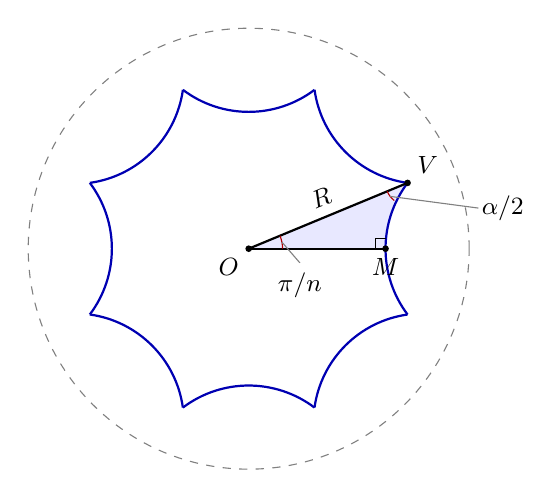
\begin{tikzpicture}[font=\small]
	\pgfmathsetmacro{\PlotRadius}{2.8}
	\pgfmathsetmacro{\VertexRadius}{.78}
	\pgfmathsetmacro{\HalfAngle}{22.5}
	\pgfmathsetmacro{\CircleCenter}{(1+\VertexRadius^2)/(2*\VertexRadius*cos(\HalfAngle))}
	\pgfmathsetmacro{\CircleRadius}{sqrt(\CircleCenter^2-1)}
	\pgfmathsetmacro{\ArcAngle}{atan2(\VertexRadius*sin(\HalfAngle),\CircleCenter-\VertexRadius*cos(\HalfAngle))}
	\pgfmathsetmacro{\Midpoint}{\PlotRadius*(\CircleCenter-\CircleRadius)}
	\coordinate (O) at (0,0);
	\coordinate (M) at (\Midpoint,0);
	\coordinate (V) at ({\PlotRadius*\VertexRadius*cos(\HalfAngle)},{\PlotRadius*\VertexRadius*sin(\HalfAngle)});
	\fill[blue!9] (O)--(M) arc[start angle=180,end angle={180-\ArcAngle},radius={\PlotRadius*\CircleRadius}]--cycle;
	\draw[dashed,gray] (O) circle (\PlotRadius);
	\foreach \j in {0,...,7}{
		\pgfmathsetmacro{\MiddleAngle}{45*\j}
		\draw[thick,blue!70!black] ({\PlotRadius*\VertexRadius*cos(\MiddleAngle-\HalfAngle)},{\PlotRadius*\VertexRadius*sin(\MiddleAngle-\HalfAngle)}) arc[start angle={\MiddleAngle+180+\ArcAngle},end angle={\MiddleAngle+180-\ArcAngle},radius={\PlotRadius*\CircleRadius}];
	}
	\draw[thick] (O)--(M);
	\draw[thick] (O)--node[midway,above,sloped] {\(R\)}(V);
	\draw (\Midpoint-.13,0)--(\Midpoint-.13,.13)--(\Midpoint,.13);
	\draw[red!70!black] (.43,0) arc[start angle=0,end angle=\HalfAngle,radius=.43];
	\node[below] at (.65,-.18) {\(\pi/n\)};
	\draw[thin,gray] (.65,-.18)--({.43*cos(\HalfAngle/2)},{.43*sin(\HalfAngle/2)});
	\begin{scope}[shift={(V)}]
		\draw[red!70!black] ({.28*cos(180+\HalfAngle)},{.28*sin(180+\HalfAngle)}) arc[start angle={180+\HalfAngle},end angle={270-\ArcAngle},radius=.28];
		\draw[thin,gray] ({.28*cos((450+\HalfAngle-\ArcAngle)/2)},{.28*sin((450+\HalfAngle-\ArcAngle)/2)})--(.9,-.32);
		\node[right,fill=white,inner sep=1pt] at (.9,-.32) {\(\alpha/2\)};
	\end{scope}
	\foreach \p in {O,M,V}{\fill (\p) circle (1.2pt);}
	\node[below left] at (O) {\(O\)};
	\node[below] at (M) {\(M\)};
	\node[above right] at (V) {\(V\)};
\end{tikzpicture}

	\caption[正则双曲多边形的直角三角形]{圆盘模型中的正则八边形。中心 \(O\)、边中点 \(M\) 与顶点 \(V\) 构成直角三角形，\(OV=R\)，中心角为 \(\pi/n\)，顶点角为 \(\alpha/2\)。虚线圆周是理想边界；测地边向圆盘中心一侧弯曲。}
	\label{g1:fig:regular-hyperbolic-polygon}
\end{figure}

角条件在粘合时有直接含义。若若干多边形顶点被识别成一个点，它们围出的角必须合计 \(2\pi\)，才可能成为普通光滑曲面点；否则会留下圆锥型的角亏或角盈。上面的 \(4g\) 个角之和正是 \(2\pi\)，而边长相等允许按保向等距匹配有序端点。下一节还会逐项检查边两侧的光滑接合、顶点邻域以及整体商空间；这里的多边形构造提供了所需的具体长度与角度数据。
